\documentclass[tikz,border=8pt]{standalone}
\usepackage{lmodern}\usetikzlibrary{arrows.meta,positioning,fit,backgrounds}
\definecolor{aws}{HTML}{EAF2F8}\tikzset{box/.style={draw,rounded corners,fill=aws,minimum width=34mm,minimum height=12mm,align=center,font=\sffamily\scriptsize},client/.style={box,fill=black!5},edge/.style={-{Latex[length=1.8mm]},thick,font=\sffamily\tiny,align=center}}
\begin{document}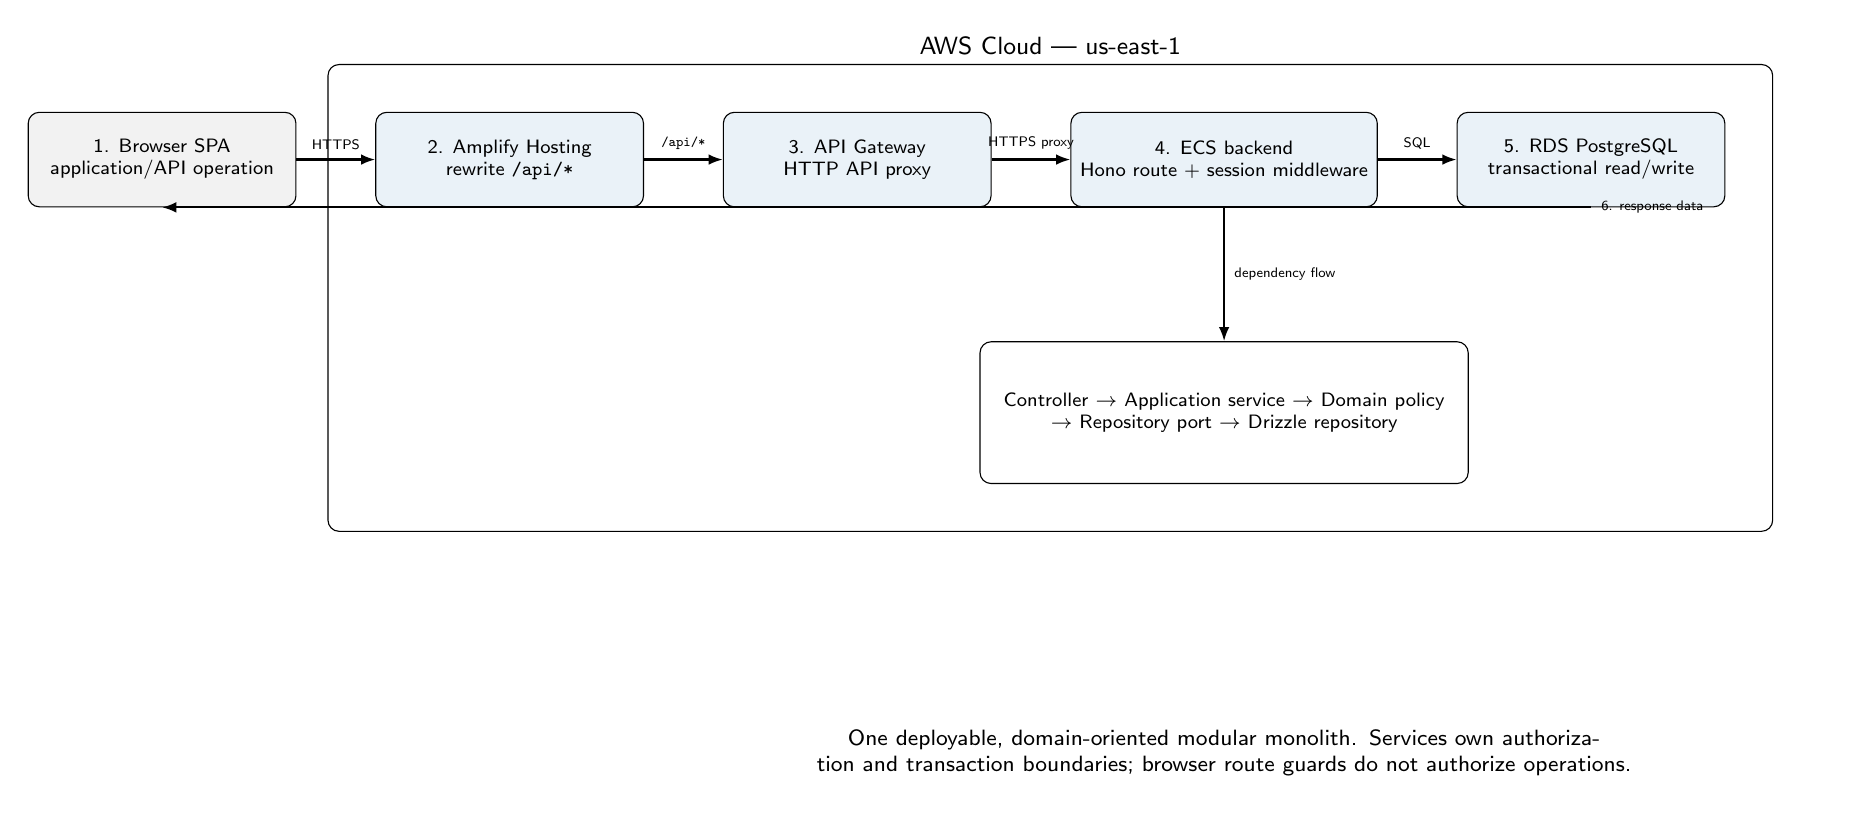
\begin{tikzpicture}[node distance=8mm and 10mm]
\node[client] (spa) {1. Browser SPA\\application/API operation};
\node[box,right=of spa] (hosting) {2. Amplify Hosting\\rewrite \texttt{/api/*}};
\node[box,right=of hosting] (gateway) {3. API Gateway\\HTTP API proxy};
\node[box,right=of gateway] (ecs) {4. ECS backend\\Hono route + session middleware};
\node[box,right=of ecs] (rds) {5. RDS PostgreSQL\\transactional read/write};
\node[draw,rounded corners,fill=white,below=17mm of ecs,minimum width=62mm,minimum height=18mm,align=center,font=\sffamily\scriptsize] (layers) {Controller $\rightarrow$ Application service $\rightarrow$ Domain policy\\$\rightarrow$ Repository port $\rightarrow$ Drizzle repository};
\draw[edge] (spa) -- node[above]{HTTPS} (hosting);\draw[edge] (hosting) -- node[above]{\texttt{/api/*}} (gateway);\draw[edge] (gateway) -- node[above]{HTTPS proxy} (ecs);\draw[edge] (ecs) -- node[above]{SQL} (rds);\draw[edge] (rds.south) |- node[pos=.25,right]{6. response data} (spa.south);
\draw[edge] (ecs) -- node[right]{dependency flow} (layers);
\begin{scope}[on background layer]\node[draw,rounded corners,fit=(hosting)(gateway)(ecs)(rds)(layers),inner sep=6mm,label={[font=\sffamily\small]above:AWS Cloud --- us-east-1}] {};\end{scope}
\node[font=\sffamily\footnotesize,align=center,text width=150mm,below=30mm of layers] {One deployable, domain-oriented modular monolith. Services own authorization and transaction boundaries; browser route guards do not authorize operations.};
\end{tikzpicture}\end{document}
